\chapter{Changing a representation without losing correctability}\label{ch:migration}

A representation can be sufficient for yesterday's questions and insufficient for today's. The old theorem need not be false. Its target may have changed. A revision procedure must therefore distinguish two tasks: translating information already retained and acquiring information that the old record discarded.

The simplest exact model makes this distinction precise. It also gives a constructive lower bound on the extra information required when a direct migration is impossible.

\section{A migration map exists exactly on constant fibres}
Let $H$ be a finite nonempty set of possible source histories. A history may include a model tag or a past observation whose value must remain available for later correction. Let
\[
 M:H\to U,\qquad N:H\to V
\]
be the old record and the required new record. Work on their attained images $U_0=M(H)$ and $V_0=N(H)$. The new record must be specified before sufficiency is claimed. It can be an answer, a correction signature, or the complete profile of future outputs in a declared finite contract.

\begin{theorem}[Exact migration criterion]\label{r:migration}
There is a map $J:U_0\to V_0$ satisfying $JM=N$ if and only if
\[
 M(h)=M(h')\quad\Longrightarrow\quad N(h)=N(h')
 \qquad(h,h'\in H).
\]
When it exists, $J$ is unique on attained old records.
\end{theorem}
\begin{proof}
Necessity follows by applying $J$ to the equal old records. Conversely, define $J(M(h))=N(h)$. The fibre condition makes the definition independent of the representative. Every $u\in U_0$ has such a representative, so the same equation determines $J$ uniquely.
\end{proof}

\source{This is the attained-record factorization of Proposition~\ref{r:factor}, applied to a representation revision. Grounded Abstraction [GA] supplies the correction-memory and evidence-migration setting. The argument does not assert a separate novelty claim for the fibre criterion.}

A collision with unequal new records is a complete obstruction to an exact deterministic migration from the old record alone. Adding more computation cannot distinguish the two histories. A randomized translator cannot be certainly correct on both either: the same old input gives the same output law, which cannot be concentrated at two different required values.

\section{What additional evidence must provide}
Suppose an allowed observation produces $E:H\to W$. A translator can use the pair $(M(h),E(h))$ rather than $M(h)$ alone.

\begin{corollary}[Evidence-assisted migration]\label{r:migration-evidence}
An exact translator from the available pair $(M,E)$ to $N$ exists if and only if
\[
 M(h)=M(h'),\ E(h)=E(h')\quad\Longrightarrow\quad N(h)=N(h').
\]
If a collision remains after the observation, that particular evidence interface cannot support the requested migration.
\end{corollary}
\begin{proof}
Apply Theorem~\ref{r:migration} to the record $h\mapsto(M(h),E(h))$.
\end{proof}

This result does not choose a physical observation or show that the observation is affordable. It tests the information supplied by a specified observation. A protocol with several actions can be treated similarly once its complete attained transcript is defined. Its admissibility, state changes, and costs then require the controller analysis of Chapter~\ref{ch:inquiry}.

\section{The least joint refinement}
When both the old and new uses must remain available, retain
\[
 P(h)=(M(h),N(h))\in P(H).
\]
The projections recover each record. No ordering between the old and new information is required.

\begin{proposition}[Universal property of the joint record]\label{r:joint-refinement-record}
If a record $R:H\to W$ determines both $M$ and $N$, then it determines $P$. In particular, $|R(H)|\ge |P(H)|$. The pair record attains this lower bound among records required to preserve both uses.
\end{proposition}
\begin{proof}
Let $fR=M$ and $gR=N$ on $H$. Then $w\mapsto(f(w),g(w))$ maps every attained value of $R$ to the corresponding attained pair. This map is onto $P(H)$, since every pair comes from a source history. Finiteness gives the cardinality inequality. The record $P$ itself has the required two projection maps.
\end{proof}

This is a statement about distinct attained values, not the byte size of a particular data structure. It allows the new state to discard duplicated encodings while preserving both information contracts.

\begin{theorem}[Minimum fixed-length supplementary information]\label{r:migration-bits}
For $u\in U_0$, put
\[
 k(u)=|N(M^{-1}\{u\})|,\qquad k_* =\max_{u\in U_0}k(u).
\]
Suppose an auxiliary encoder may inspect the complete source history and sends one fixed-length binary word in addition to the old record. Exact recovery of $N$ is possible with $b$ supplementary bits if and only if $2^b\ge k_*$. Thus the minimum is $\lceil\log_2 k_*\rceil$.
\end{theorem}
\begin{proof}
For a fixed old record $u$, distinct required new values must receive distinct supplementary words. Otherwise the decoder would receive identical inputs with different required outputs. Hence $2^b\ge k(u)$ for every $u$.

Conversely, within each old fibre assign distinct binary words to the distinct attained new values, using at most $k_*\le 2^b$ words. The same word can be reused in different old fibres because the decoder receives $u$ as well. Define the encoder by this fibre-specific table and decode by the inverse table. Every source history is recovered correctly.
\end{proof}

The encoder's access assumption is essential. The bound does not allow a controller holding only $M(h)$ to manufacture the missing bits. It describes the amount of supplementary information when an encoder actually has the source information. With restricted observations, Corollary~\ref{r:migration-evidence} must be checked first. Code tables, acquisition, transmission, and validation also carry costs not counted by the fixed binary payload.

\section{Migration must commute with subsequent operations}
Recovering one new record is not yet preserving a method. Let a common finite action alphabet act on $H$ through total maps $F_a:H\to H$. Suppose both representations close under those same source operations:
\[
 M F_a=P_a M,\qquad N F_a=Q_a N.
\]
The maps $P_a$ and $Q_a$ preserve the attained record sets. These equations refer to the same source action, not merely to operations sharing a name.

\begin{theorem}[A valid migration intertwines the common operations]\label{r:migration-operations}
If $JM=N$, then on $U_0$,
\[
 JP_a=Q_aJ.
\]
Consequently $JP_w=Q_wJ$ for every finite action word $w$, with the execution-order convention of Chapter~\ref{ch:evidence}. Any protected readout that factors through $N$ agrees along the two migrated executions.
\end{theorem}
\begin{proof}
Take $u=M(h)$. Then
\[
 JP_a(u)=JM(F_a h)=N(F_a h)=Q_aN(h)=Q_aJ(u).
\]
Every attained $u$ has a representative, so the equality holds throughout $U_0$. Closure keeps later values within that domain. Induction on the word length gives the continuation identity. Composing with the protected readout gives equality of outputs.
\end{proof}

If a revision changes the underlying operation, the second closure equation must be proved for the changed semantics. A successful initial decoding does not imply it. For example, the identity translator on a bit preserves its current value, but cannot intertwine an old hold operation with a new flip operation. The same stored bit and the same printed operation name do not supply the missing commuting equation.

\section{A worked change of task}
Use the eight histories $(b,s,n)\in\{0,1\}^3$ and the old display record $M=b\oplus s$. For display prediction under physical-bit flips, this record is sufficient. Suppose the new task requires both the display and the physical target, so $N=(b\oplus s,b)$.

There are two possible new records inside each old display fibre. Direct migration fails, but $k_*=2$, so one supplementary bit is information-theoretically sufficient. Calibration supplies $E=s$, and
\[
 b=M\oplus E
\]
gives the actual decoder. The joint old/new record has four attained states. The nuisance bit remains discarded because the new task still does not use it.

Now require the nuisance bit as well. The new record $N'=(b\oplus s,b,n)$ has four possible values inside each old fibre, giving a two-bit supplementary lower bound. Calibration alone no longer suffices. Two histories with equal $b,s$ and different $n$ collide under $(M,E)$ but have different $N'$. The lower bound identifies a missing distinction rather than a computational bottleneck.

\begin{figure}[htbp]\centering
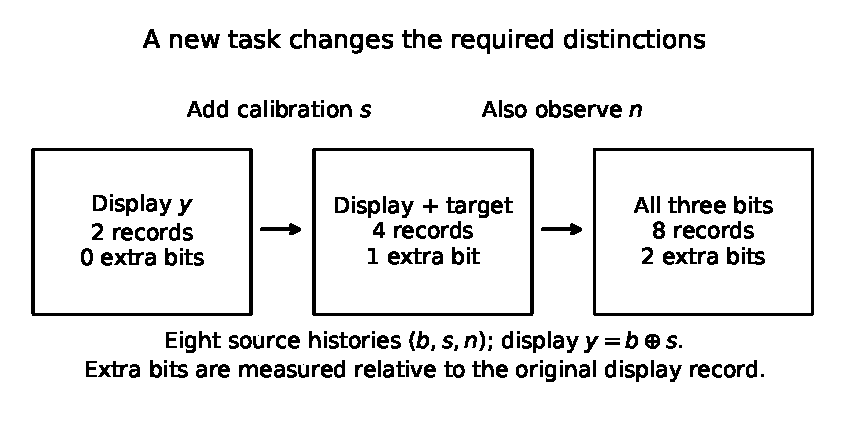
\includegraphics[width=.93\linewidth]{figures/migration_fibres.pdf}
\caption{The required information depends on the revised task. Display alone has two attained values. Adding the target bit requires four joint values. Adding the nuisance bit requires eight. Calibration supplies the first missing distinction, not the second.}\label{fig:migration-fibres}
\end{figure}

\section{Certificates after a change of contract}
A migration map transports data. A certificate authorizes a conclusion only relative to its premises. To reuse a certificate across a revision, specify an old predicate $\varphi$ on $U_0$, a new predicate $\psi$ on $V_0$, and a proved implication
\[
 \varphi(u)\ \Longrightarrow\ \psi(Ju).
\]
An old witness for $\varphi(u)$ and this implication then yield the new conclusion. The implication may express semantic preservation, a stronger guard, or a deliberately weaker postcondition. It cannot be replaced by equality of file names or by an unchanged serialization format.

Chapter~\ref{ch:revision} handles the dependency graph needed to know which such implications remain applicable. The present chapter handles information loss and operation transport. Together they separate three questions that a revision must answer: can the new record be recovered, does it support the required operations, and do the old proof premises still justify the intended conclusions?
